\documentclass{article}

% If you're new to LaTeX, here's some short tutorials:
% https://www.overleaf.com/learn/latex/Learn_LaTeX_in_30_minutes
% https://en.wikibooks.org/wiki/LaTeX/Basics

% Formatting
\usepackage[utf8]{inputenc}
\usepackage[margin=1in]{geometry}
\usepackage[titletoc,title]{appendix}

% Math
% https://www.overleaf.com/learn/latex/Mathematical_expressions
% https://en.wikibooks.org/wiki/LaTeX/Mathematics
\usepackage{amsmath,amsfonts,amssymb,mathtools}

% Images
% https://www.overleaf.com/learn/latex/Inserting_Images
% https://en.wikibooks.org/wiki/LaTeX/Floats,_Figures_and_Captions
\usepackage{graphicx,float}
\usepackage[utf8]{inputenc}

% Tables
% https://www.overleaf.com/learn/latex/Tables
% https://en.wikibooks.org/wiki/LaTeX/Tables

% Algorithms
% https://www.overleaf.com/learn/latex/algorithms
% https://en.wikibooks.org/wiki/LaTeX/Algorithms
\usepackage[ruled,vlined]{algorithm2e}
\usepackage{algorithmic}

% Code syntax highlighting
% https://www.overleaf.com/learn/latex/Code_Highlighting_with_minted
\usepackage{minted}
\usemintedstyle{borland}

% Title content
\title{ECON 5253 Problem Set 4}
\author{Ahmed Chaudhry}
\date{\today}

\begin{document}
\maketitle
\section{Question No. 3}
I downloaded the State House/Assembly and Senate Campaign Contributions data at the state level for the election years between 1998 to 2014 from the Institute of Money in Politics's website. This data was then cleaned in R.
 
,In order to perform the data cleaning task, I first deleted the unnecessary columns/variables. Then to ease the interpretation of campaign contribution amounts, I re-scaled the total amount to million USDs, followed by generating two new variables with each representing contributions in million USD's to State House/Assembly and State Senate, respectively. Next, I dropped the years in which elections were not held, and then finally, I generated three plots which are described in Q4. 
\section{Question No. 4 \& 5}
\begin{figure}[htp]
    \centering
    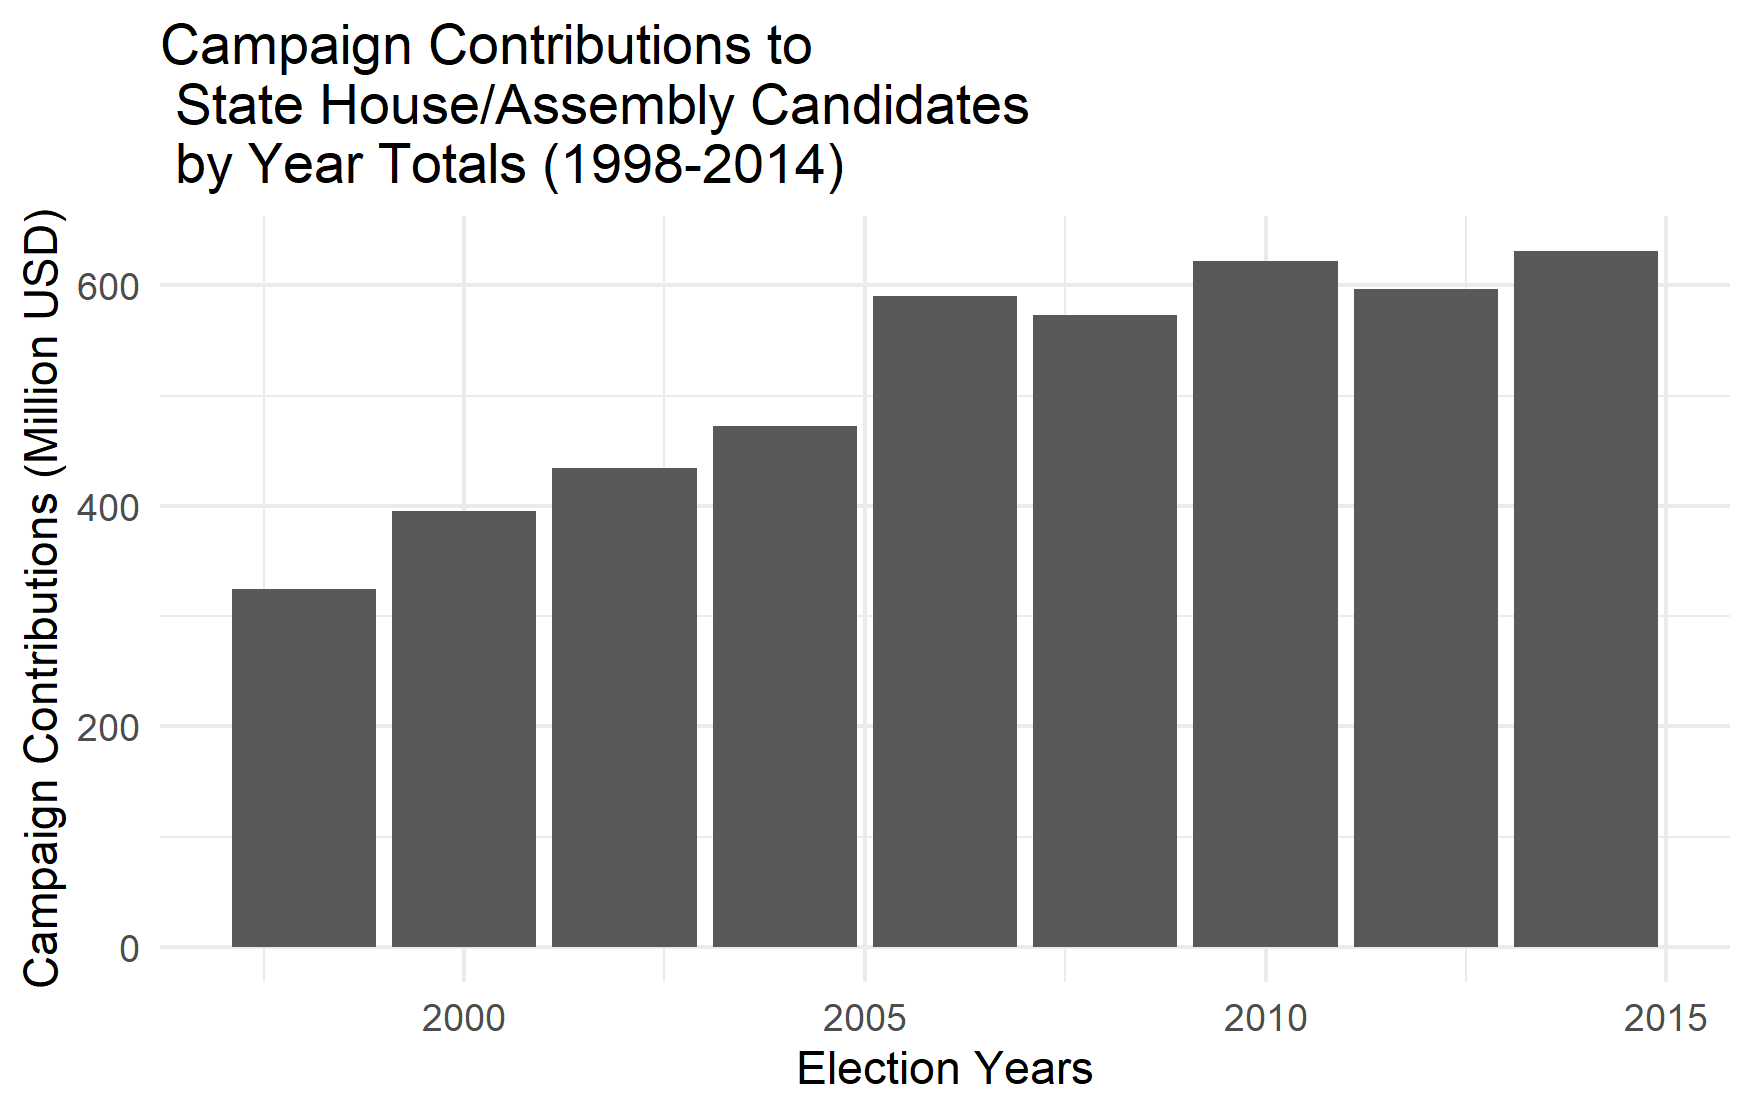
\includegraphics[]{PS6a_Chaudhry.png}
\end{figure}

This first histogram shows state totals (in million USDs) of campaign contributions to state house/assembly candidates in different elections years. It can be seen that there is an increasing trend of money in politics. In 1998, the total contributions to state house candidates amounted to about USD 315 million, which doubled to about USD 610 million in 2014.

\begin{figure}[htp]
    \centering
    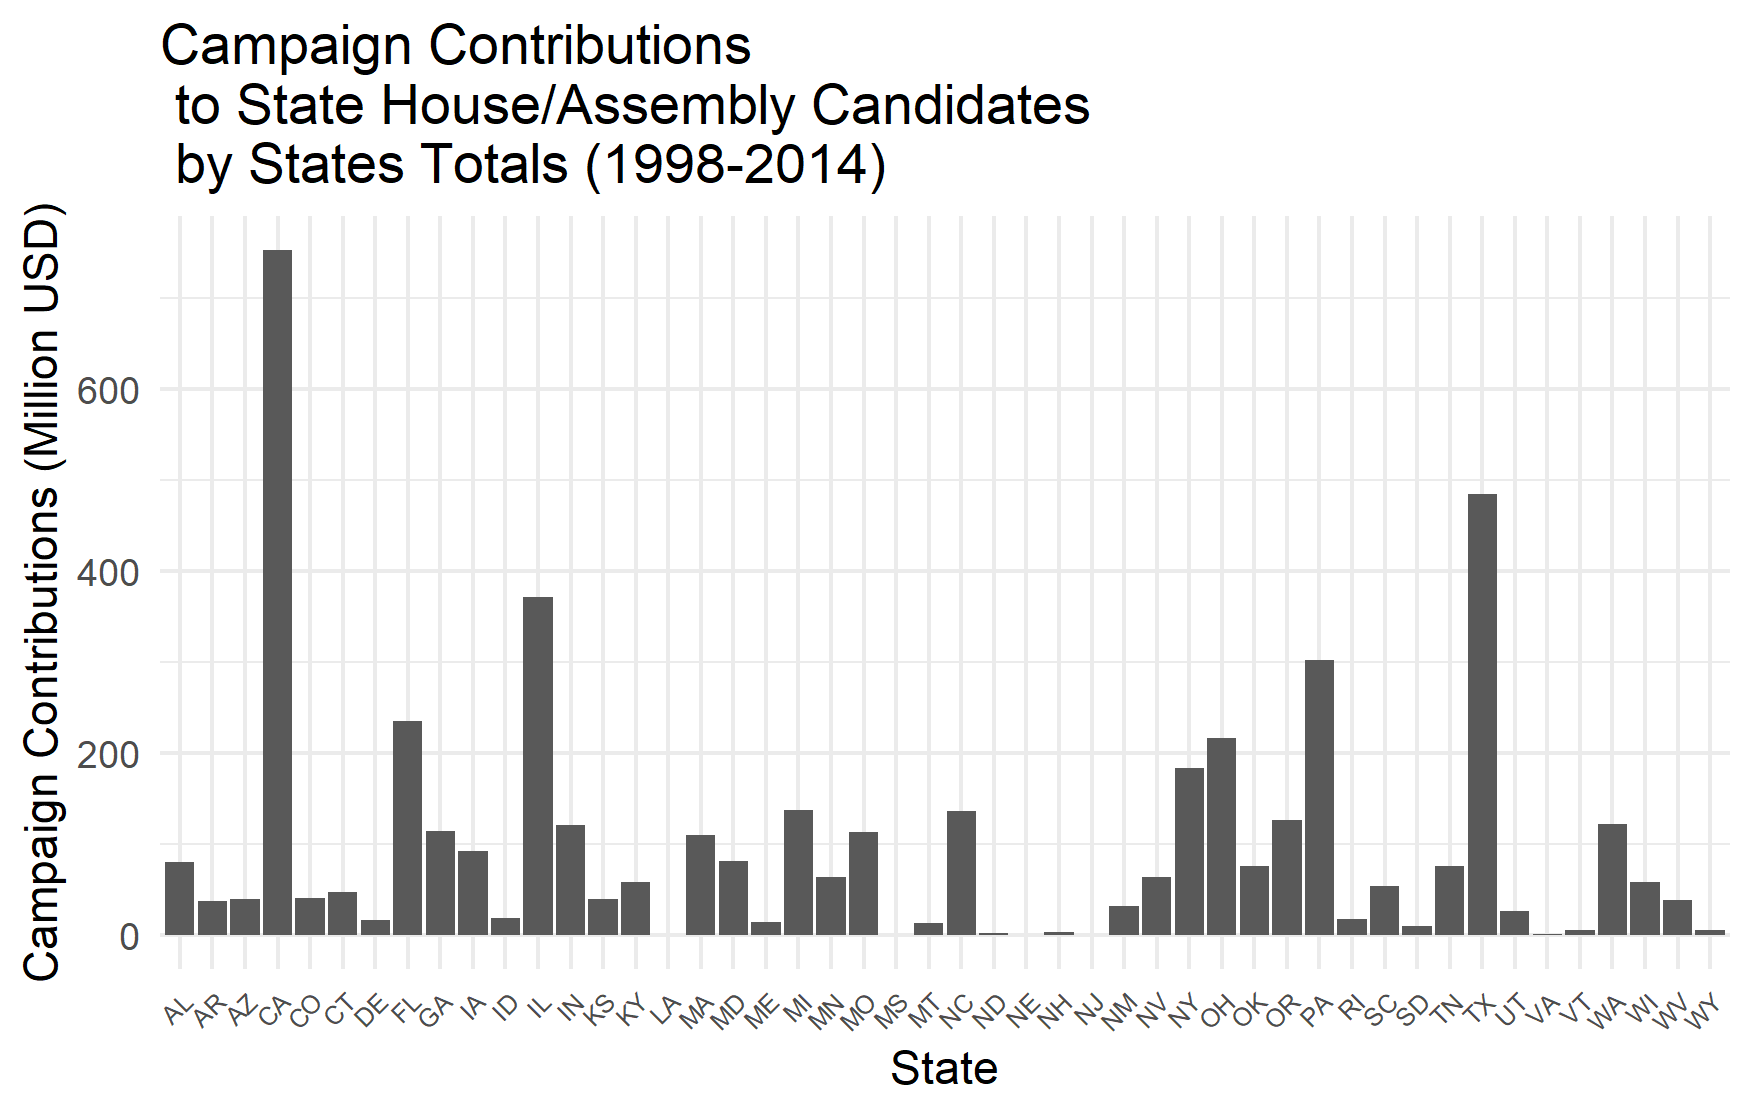
\includegraphics[]{PS6b_Chaudhry.png}
\end{figure} 
I then wanted to see the total contributions in each state over the entire time period (1998-2014). The 2nd graph shows that California stands as an outlier for having enormous amount of total campaign contributions, reaching more than USD 700 million in the given 17 year period.

\begin{figure}[htp]
    \centering
    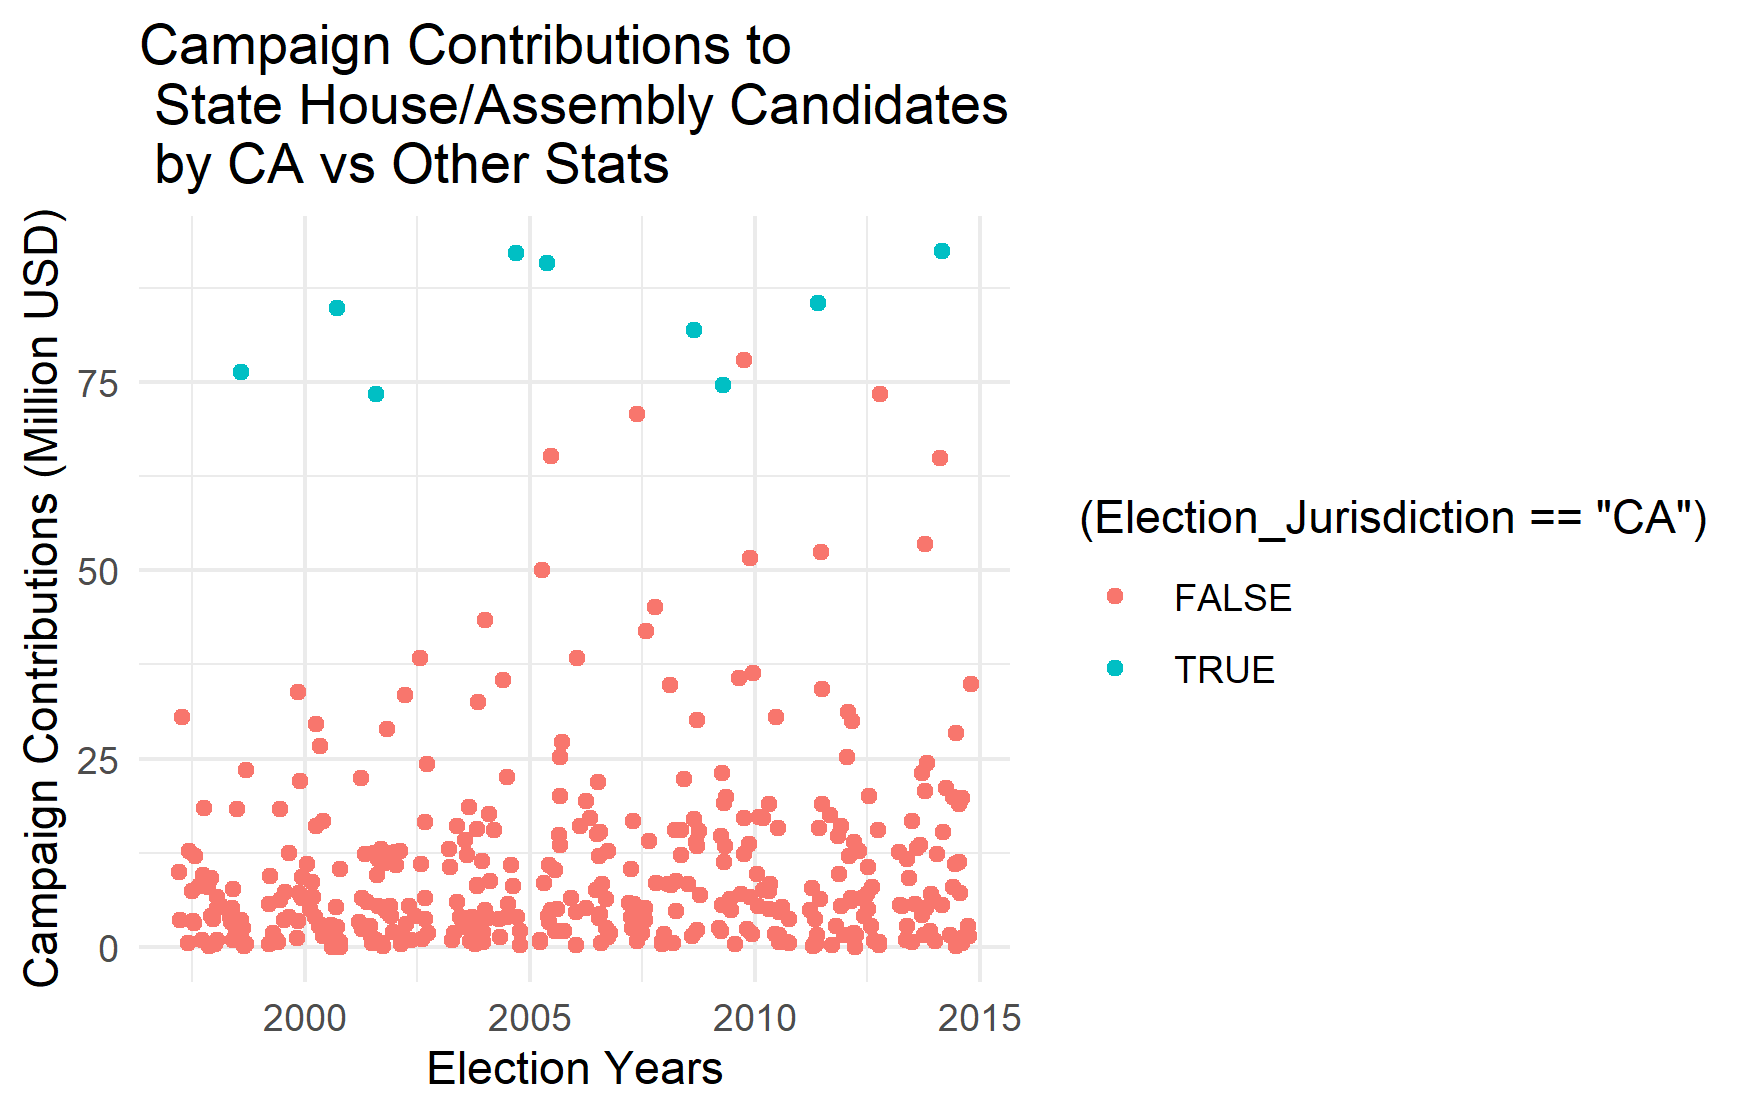
\includegraphics[height=7.5cm]{PS6c_Chaudhry.png}
\end{figure}

Graph 2 got me curious, so I got interested to see how the trend of campaign contributions in California (CA) is varying overtime as compared to the rest of the states, as captured in graph 3. It seems that the state house candidates in California are consistently doing better in terms of the amount of donations they gathered.

\end{document}

